\chapter{Multiplication II: the number-theoretic transform}
\label{ch:ntt}

For large numbers BigMath multiplies with a \emph{number-theoretic transform} (NTT), a
version of the fast Fourier transform (FFT) that works with whole numbers modulo a prime
instead of floating-point complex numbers. Its cost grows like $n \log n$, so it beats
every method of \cref{ch:mul} once the numbers are large enough. This chapter builds it up
in steps: first what has to be computed, then why a transform helps, then the tricks that
make BigMath's implementation fast.

\section{Multiplication is a convolution}

Treat each number as a list of digits. When you multiply, digit position $k$ of the
answer (before carrying) collects every product $a_i b_j$ with $i + j = k$:
\[
c_k = \sum_{i + j = k} a_i\, b_j .
\]
This sum-over-diagonals is called a \emph{convolution}. Carrying comes afterwards.

\begin{example}[: $12 \times 34$ as a convolution]
Little-endian digits: $a = (2, 1)$, $b = (4, 3)$.
\begin{align*}
c_0 &= a_0 b_0 = 8\\
c_1 &= a_0 b_1 + a_1 b_0 = 6 + 4 = 10\\
c_2 &= a_1 b_1 = 3
\end{align*}
Now carry: $c_1 = 10$ becomes digit 0 with a carry of 1 into $c_2$, giving digits
$(8, 0, 4)$, that is $408 = 12 \times 34$.
\end{example}

Computing the convolution directly is schoolbook multiplication again: $n^2$ products.
The FFT idea is to compute it a completely different way.

\section{Why a transform helps}

\Cref{sec:toom} showed the recipe ``evaluate at some points, multiply the values
pointwise, interpolate''. A product with $N$ coefficients needs $N$ points. Pointwise
multiplication then costs only $N$ multiplications. The problem is the evaluation and
interpolation: at arbitrary points they cost about $N^2$ each, which gains nothing.

The FFT fixes this by choosing very special points: the $N$-th \emph{roots of unity}, the
$N$ numbers $\omega^0, \omega^1, \dots, \omega^{N-1}$ where $\omega^N = 1$. Their powers
repeat in a pattern that lets an evaluation of size $N$ be split into two evaluations of
size $N/2$, which split again, and so on. That divide-and-conquer brings evaluation down
to about $N \log_2 N$ operations.

\begin{figure}[ht]
\centering
\begin{tikzpicture}[node distance=6mm and 9mm]
  \node[box,fill=sOrange!12] (a) {digits of $a$};
  \node[box,fill=sOrange!12,below=of a] (b) {digits of $b$};
  \node[box,right=of a] (fa) {forward\\transform};
  \node[box,right=of b] (fb) {forward\\transform};
  \node[box,fill=paper,right=18mm of $(fa)!0.5!(fb)$] (pw) {multiply\\point by point};
  \node[box,right=of pw] (inv) {inverse\\transform};
  \node[box,right=of inv] (car) {carry};
  \node[box,fill=sOrange!12,right=of car] (out) {$a\cdot b$};
  \draw[arr] (a) -- (fa); \draw[arr] (b) -- (fb);
  \draw[arr] (fa) -- (pw); \draw[arr] (fb) -- (pw);
  \draw[arr] (pw) -- (inv); \draw[arr] (inv) -- (car); \draw[arr] (car) -- (out);
  \node[lbl,below=1mm of inv] {$N\log N$};
  \node[lbl,below=1mm of pw] {$N$};
  \node[lbl,below=1mm of fb] {$N\log N$ each};
\end{tikzpicture}
\caption{Transform-based multiplication: three transforms, one cheap pointwise pass, one
carry pass.}
\end{figure}

\subsection{Why modulo a prime?}

The textbook FFT uses complex numbers such as $e^{2\pi i/N}$, computed in floating point.
Rounding errors then make it hard to guarantee exact integer results for very large
inputs. In arithmetic modulo a suitable prime $P$ there are also numbers with
$\omega^N = 1$, and every calculation is exact. The transform computes each $c_k$ modulo
$P$; if $P$ is larger than any possible $c_k$, that \emph{is} $c_k$.

\begin{example}[: a complete NTT by hand, modulo 17]
Multiply $12 \times 34$ again, with $N = 4$ points modulo $P = 17$. The number
$\omega = 4$ works as a 4th root of unity: $4^2 = 16 \equiv -1$ and $4^4 \equiv 1 \pmod{17}$.
Its powers are $\omega^0 = 1,\ \omega^1 = 4,\ \omega^2 = 16,\ \omega^3 = 13$.

\textbf{Forward transform}: $A_k = \sum_j a_j\, \omega^{jk} \bmod 17$, with $a = (2,1,0,0)$
and $b = (4,3,0,0)$ padded to length 4:
\begin{center}
\begin{tabular}{lcccc}
\toprule
$k$ & 0 & 1 & 2 & 3 \\
\midrule
$A_k$ & $2+1 = 3$ & $2+4 = 6$ & $2+16 \equiv 1$ & $2+13 \equiv 15$ \\
$B_k$ & $4+3 = 7$ & $4+12 = 16$ & $4+48 \equiv 1$ & $4+39 \equiv 9$ \\
$C_k = A_k B_k$ & $21 \equiv 4$ & $96 \equiv 11$ & $1$ & $135 \equiv 16$ \\
\bottomrule
\end{tabular}
\end{center}

\textbf{Inverse transform}: $c_j = N^{-1} \sum_k C_k\, \omega^{-jk}$. Here $N^{-1} = 4^{-1} = 13$
(since $4 \cdot 13 = 52 \equiv 1$) and the inverse powers are $\omega^{-1} = 13$,
$\omega^{-2} = 16$, $\omega^{-3} = 4$:
\begin{align*}
c_0 &= 13\,(4 + 11 + 1 + 16) = 13 \cdot 32 \equiv 8\\
c_1 &= 13\,(4 + 11\cdot 13 + 1 \cdot 16 + 16 \cdot 4) = 13 \cdot 227 \equiv 10\\
c_2 &= 13\,(4 + 11 \cdot 16 + 1 + 16 \cdot 16) = 13 \cdot 437 \equiv 3\\
c_3 &= 13\,(4 + 11 \cdot 4 + 1 \cdot 16 + 16 \cdot 13) = 13 \cdot 272 \equiv 0
\end{align*}
The result $(8, 10, 3, 0)$ is exactly the convolution from the previous example. Carrying
gives 408.
\end{example}

\subsection{Wrap-around: the transform length must be long enough}

A length-$N$ transform computes the convolution \emph{cyclically}: coefficients past
position $N-1$ wrap around and are added to the start. In the language of polynomials it
computes the product modulo $x^N - 1$. That is why the transform must be at least as long
as the product: with $N = 2$ above, $c_2 = 3$ would have landed on top of $c_0$.

\begin{another}[: wrap-around is not always a bug]
With $N = 2$ the transform gives $(c_0 + c_2,\ c_1) = (11, 10)$, which reads as
$11 + 10 \cdot 10 = 111$. That is not $408$, but it \emph{is} $408$ modulo $10^2 - 1 = 99$
($408 = 4 \cdot 99 + 12$ and $111 = 99 + 12$). In general a cyclic transform of length $L$
computes a product modulo $B^L - 1$ at half the price of the full product. Newton division
uses exactly this (\cref{sec:wrap}): when only the low part of a product is needed, a
wrapped product is enough.
\end{another}

\section{The butterfly: how the transform is fast}

The forward transform of length $N$ splits into two transforms of length $N/2$, joined by
$N/2$ \emph{butterflies}. A butterfly takes two values $u, v$ and a twiddle factor $w$
(a power of $\omega$) and produces $u + v$ and $(u - v)\,w$. After $\log_2 N$ layers of
butterflies the transform is done.

\begin{figure}[ht]
\centering
\begin{tikzpicture}[x=2.3cm,y=0.62cm]
  \foreach \s in {0,1,2,3} \foreach \i in {0,...,7} \fill[ink2] (\s,-\i) circle (1.6pt);
  \foreach \i in {0,...,7} \node[lbl,anchor=east] at (-0.1,-\i) {$x_\i$};
  % stage 1: span 4
  \foreach \i in {0,...,3} {
    \pgfmathtruncatemacro{\j}{\i+4}
    \draw[sBlue] (0,-\i) -- (1,-\i); \draw[sBlue] (0,-\j) -- (1,-\j);
    \draw[sBlue] (0,-\i) -- (1,-\j); \draw[sBlue] (0,-\j) -- (1,-\i);
  }
  % stage 2: span 2
  \foreach \b in {0,4} \foreach \o in {0,1} {
    \pgfmathtruncatemacro{\i}{\b+\o} \pgfmathtruncatemacro{\j}{\b+\o+2}
    \draw[sViolet] (1,-\i) -- (2,-\i); \draw[sViolet] (1,-\j) -- (2,-\j);
    \draw[sViolet] (1,-\i) -- (2,-\j); \draw[sViolet] (1,-\j) -- (2,-\i);
  }
  % stage 3: span 1
  \foreach \b in {0,2,4,6} {
    \pgfmathtruncatemacro{\j}{\b+1}
    \draw[sOrange] (2,-\b) -- (3,-\b); \draw[sOrange] (2,-\j) -- (3,-\j);
    \draw[sOrange] (2,-\b) -- (3,-\j); \draw[sOrange] (2,-\j) -- (3,-\b);
  }
  \node[lbl] at (0.5,1) {layer 1}; \node[lbl] at (1.5,1) {layer 2}; \node[lbl] at (2.5,1) {layer 3};
  \begin{scope}[shift={(4.0,-2.2)}]
    \node[box,minimum width=6mm] (u) at (0,0.9) {$u$};
    \node[box,minimum width=6mm] (v) at (0,-0.9) {$v$};
    \node[box,minimum width=16mm,anchor=west] (s) at (1.0,0.9) {$u + v$};
    \node[box,minimum width=16mm,anchor=west] (d) at (1.0,-0.9) {$(u - v)\cdot w$};
    \draw[arr] (u) -- (s.west); \draw[arr] (v) -- (d.west);
    \draw[arr] (u) -- (d.west); \draw[arr] (v) -- (s.west);
    \node[lbl] at (0.8,2.4) {one butterfly};
  \end{scope}
\end{tikzpicture}
\caption{A length-8 transform: three layers of four butterflies each. In general
$\log_2 N$ layers of $N/2$ butterflies, so about $\tfrac12 N\log_2 N$ modular
multiplications.}
\label{fig:butterfly}
\end{figure}

\subsection{Fewer passes over memory: radix-4 and radix-8}

Each layer in \cref{fig:butterfly} reads and writes the whole array once. For large
transforms the array does not fit in cache, so each pass is a trip to main memory.
BigMath fuses three layers into one \emph{radix-8} step: it loads 8 values, does all 12
butterflies of those three layers in registers, and writes 8 values back. The arithmetic
is unchanged, but the number of passes over memory drops by a factor of three. One or two
leftover layers are handled by radix-4 or radix-2 steps. This alone gave about 1.5 times
on large products.

\subsection{No reordering pass}

A textbook FFT has to permute its data into ``bit-reversed'' order before or after the
butterflies. BigMath avoids this: the forward transform is written so that it
\emph{leaves} the output in bit-reversed order (decimation in frequency), and the inverse
is written to \emph{accept} bit-reversed input and produce natural order (decimation in
time). Both operands are scrambled the same way, so the pointwise multiplication still
lines up. The permutation pass simply disappears (about 15\% saved).

\section{Three primes and the Chinese remainder theorem}
\label{sec:crt}

How large can a convolution coefficient get? BigMath splits each 64-bit limb into two
32-bit coefficients. A product coefficient is a sum of up to $N$ products of two 32-bit
numbers, so it can approach $N \cdot 2^{64}$. For $N = 2^{26}$ that is about $2^{90}$: far
larger than any 32-bit or even 64-bit prime.

Instead of one huge prime, the library uses three primes that each fit in 31 bits, and
computes the whole convolution three times, once modulo each:

\begin{center}
\begin{tabular}{rrc}
\toprule
prime & form & longest transform \\
\midrule
$P_1 = 2\,013\,265\,921$ & $15 \cdot 2^{27} + 1$ & $2^{27}$ \\
$P_2 = 469\,762\,049$ & $7 \cdot 2^{26} + 1$ & $2^{26}$ \\
$P_3 = 1\,811\,939\,329$ & $27 \cdot 2^{26} + 1$ & $2^{26}$ \\
\bottomrule
\end{tabular}
\end{center}

Each prime has the form $k \cdot 2^m + 1$; that is what guarantees roots of unity for every
power-of-two length up to $2^m$. Knowing a number modulo three primes determines it
modulo their product $P_1 P_2 P_3 \approx 2^{90.5}$, which is larger than any coefficient.
Recovering it is the \emph{Chinese remainder theorem}; the library uses Garner's form of it.

\begin{example}[: rebuilding 52 from its remainders mod 3, 5, 7]
Suppose we only know $x \bmod 3 = 1$, $x \bmod 5 = 2$, $x \bmod 7 = 3$, and that
$x < 3 \cdot 5 \cdot 7 = 105$. Garner builds $x = r_1 + 3\,u_2 + 15\,u_3$ one prime at a time:
\begin{itemize}
  \item Start with $r_1 = 1$.
  \item Choose $u_2$ so that the value is right mod 5: $1 + 3u_2 \equiv 2$, so
        $3u_2 \equiv 1$, so $u_2 = 2$. Now $x \equiv 7$.
  \item Choose $u_3$ so that it is right mod 7: $7 + 15u_3 \equiv 3$. Since
        $15 \equiv 1 \pmod 7$ this is $u_3 \equiv 3 - 7 \equiv 3$. Now $x = 7 + 45 = 52$.
\end{itemize}
Check: $52 = 17\cdot 3 + 1 = 10 \cdot 5 + 2 = 7 \cdot 7 + 3$.
\end{example}

The library does the same with $P_1, P_2, P_3$ for every coefficient, then adds the
$\approx 90$-bit coefficients into the output limbs with carries. This last pass is called
\emph{finalize}.

\begin{keyidea}
Three transforms with small primes are cheaper than one with a huge prime: small primes fit
in 32-bit lanes, and the three transforms are independent, so they run on different cores
at the same time.
\end{keyidea}

The largest transform is $2^{26}$ coefficients, which bounds a product at about 646 million
decimal digits; past that the library throws an exception rather than return a wrong
answer. A single-prime alternative (the ``Goldilocks'' prime $2^{64} - 2^{32} + 1$ with
16-bit pieces) is still in the source as the \code{-DBIGMATH\_NTT\_CRT=0} build, but the
three-prime version is faster at every measured size.

\begin{pitfall}
The first prime set had one prime that only supported transforms up to $2^{22}$. Above
that length the computed ``root of unity'' was not a true root, one of the three residues
was silently wrong, and products of about 22 million digits came out incorrect. It was
caught by comparing against GMP and fixed by choosing the primes above. The test suites
now compare NTT products limb for limb against Karatsuba and against GMP.
\end{pitfall}

\section{Fast modular multiplication: Shoup's trick}

Every butterfly multiplies a value $x$ by a twiddle $w$ modulo $P$. A real division by $P$
would be slow. But $w$ is fixed (it comes from a table), so the library precomputes a
companion value
\[
w' = \floor{\frac{w \cdot 2^{31}}{P}}
\]
and then computes $q = \floor{w' x / 2^{31}}$, which is $\floor{wx/P}$ or one less. The
remainder $t = wx - qP$ is then between $0$ and $2P$, and one conditional subtraction
finishes the job. No division anywhere.

\begin{example}[: Shoup multiplication with small numbers]
Use $P = 17$ and, to keep numbers small, scale by $2^8 = 256$ instead of $2^{31}$.
For $w = 5$: $w' = \floor{5 \cdot 256 / 17} = \floor{75.3} = 75$.
\begin{itemize}
  \item $x = 13$: $q = \floor{75 \cdot 13 / 256} = \floor{975/256} = 3$, and
        $t = 5 \cdot 13 - 3 \cdot 17 = 65 - 51 = 14$. Indeed $65 \bmod 17 = 14$.
  \item $x = 16$: $q = \floor{1200/256} = 4$, $t = 80 - 68 = 12 = 80 \bmod 17$.
\end{itemize}
\end{example}

On ARM processors the library runs four of these at once with NEON vector instructions.
Scaling the companion by $2^{31}$ (not the classic $2^{32}$) lets one instruction,
\code{vqdmulhq\_s32} (``doubling multiply, keep high half''), compute $q$ for four lanes.
The conditional subtraction uses an unsigned minimum: for $t \in [0, 2P)$, $\min(t, t - P)$ is
the reduced value, because $t - P$ wraps around to a huge number exactly when $t < P$.
These two changes cut a butterfly from about 19 vector instructions to 11.

\begin{perfnote}
The vector butterflies run about 4 times faster than scalar code. Twiddles and their
companions are stored interleaved, so each pair is one cache line. Special ``tail'' kernels
handle the last layers of every transform size four lanes wide, so every transform with
$N \ge 16$ is vectorized end to end. Each step was checked bit-for-bit against the plain
scalar transform for all three primes at every length from $2^1$ to $2^{16}$.
\end{perfnote}

\section{Big transforms and the cache: the matrix (six-step) method}
\label{sec:mfa}

A transform of $2^{22}$ coefficients uses 16\,MB per array, far more than the processor's
caches. Even with radix-8 fusion, each pass goes to main memory.

The \emph{matrix Fourier algorithm} (Bailey's six-step FFT) rearranges a length
$N = N_1 \times N_2$ transform as a grid:

\begin{figure}[ht]
\centering
\begin{tikzpicture}[scale=0.42]
  \foreach \r in {0,...,5} \foreach \c in {0,...,7} \draw[rule,fill=white] (\c,-\r) rectangle +(1,-1);
  \foreach \r in {0,...,5} \fill[sBlue!25] (0,-\r) rectangle (8,-\r-0.85);
  \node[lbl] at (4,1) {1. short transforms along rows};
  \begin{scope}[shift={(11,0)}]
    \foreach \r in {0,...,5} \foreach \c in {0,...,7} \draw[rule,fill=sOrange!20] (\c,-\r) rectangle +(1,-1);
    \node[lbl] at (4,1) {2. multiply by twiddles};
  \end{scope}
  \begin{scope}[shift={(22,0)}]
    \foreach \r in {0,...,5} \foreach \c in {0,...,7} \draw[rule,fill=white] (\c,-\r) rectangle +(1,-1);
    \foreach \c in {0,...,7} \fill[sViolet!25] (\c,0) rectangle (\c+0.85,-6);
    \node[lbl] at (4,1) {3. short transforms along columns};
  \end{scope}
  \draw[arr] (8.3,-3) -- (10.7,-3);
  \draw[arr] (19.3,-3) -- (21.7,-3);
\end{tikzpicture}
\caption{The matrix method: one long transform becomes many short ones that fit in cache,
plus a twiddle pass and transposes.}
\end{figure}

Each short transform (at most $2^{13}$ entries, \code{BIGMATH\_NTT\_MFA\_LEAF}) fits in the
fastest cache, so the butterflies run at cache speed. BigMath goes further and
\emph{fuses} the transposes, the packing of input limbs, and even the pointwise
multiplication into these passes, so the second operand's transform never gets written to
memory at all. The method is used from transform length $2^{20}$
(\code{BIGMATH\_NTT\_MFA\_THRESHOLD}); at $2^{22}$ it made products 3 times faster.

\section{The power-of-two staircase and the $H + L$ trick}
\label{sec:trunc}

The transform length is a power of two at least as long as the product. A product needing
$c = 4100$ coefficients therefore uses length 8192: almost double the work of a product
needing 4096. Plotted against size, the cost is a staircase (\cref{fig:trunc}).

\begin{figure}[ht]
\centering
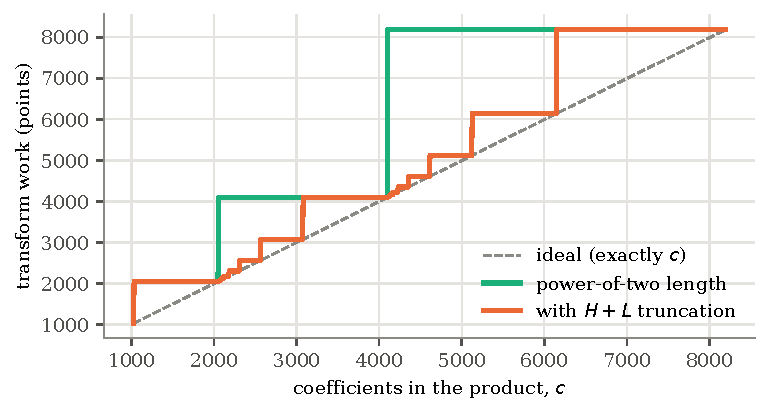
\includegraphics[width=0.8\textwidth]{figures/trunc_staircase.pdf}
\caption{Transform work against product size. Green: plain power-of-two lengths. Orange:
with the $H+L$ scheme, which fills in the steps just above each power of two (for
$2048 \le H \le 2^{20}$, up to $1.5H$). Computed from the length rules in the source.}
\label{fig:trunc}
\end{figure}

For a product just above a power of two $H$, BigMath computes it in two smaller pieces and
glues them together:

\begin{enumerate}
  \item The product \emph{modulo $x^H + 1$}, using a length-$H$ transform. (This is a
        ``negacyclic'' transform: coefficients that wrap around come back with a minus
        sign. It is a normal transform with the inputs pre-multiplied by powers of a
        $2H$-th root of unity; those weights are exactly the twiddle tables of the length-$2H$
        transform, so nothing new is needed.)
  \item The product \emph{modulo $x^L - 1$}, using a short cyclic transform of length $L$,
        the smallest power of two covering the overflow $c - H$.
\end{enumerate}

Because $x^H + 1$ and $x^L - 1$ share no factor, the two residues determine the product,
and a simple formula recovers it: if $C = C_{\text{lo}} + x^H C_{\text{hi}}$, the first
residue is $C_{\text{lo}} - C_{\text{hi}}$ and the second determines $C_{\text{hi}}$, so
$C_{\text{hi}} = (\text{second} - \text{folded first})/2$ and
$C_{\text{lo}} = \text{first} + C_{\text{hi}}$. Total transform work is $H + L$ instead of
$2H$.

\begin{center}
\small
\begin{tabular}{rrrrrr}
\toprule
$H$ & $c \approx H$ & $c = 1.0625H$ & $c = 1.125H$ & $c = 1.25H$ & full $2H$ \\
\midrule
$2^{13}$ & 87.7 & 90.5 & 95.7 & 103.7 & 143.5 \\
$2^{16}$ & 519.6 & 536.6 & 572.9 & 621.6 & 1\,132.6 \\
$2^{18}$ & 2\,891 & 3\,064 & 3\,657 & 3\,951 & 6\,839 \\
\bottomrule
\end{tabular}

\smallskip
{\footnotesize Microseconds per multiply, threaded, M1 Max.}
\end{center}

In single-threaded builds the scheme continues up to $H = 2^{25}$ for the whole octave,
processing one prime at a time to keep the working set small (0.45--0.88 times the full
transform's time). Multithreaded builds keep the full transform above $2^{20}$ because its
fused stages split better across cores.

\section{Using all the cores}
\label{sec:nttthreads}

A product needs six forward transforms (two operands times three primes), and they are
independent. BigMath runs them as six work units on its thread pool, then the pointwise
products, then the inverse transforms. Three inverse transforms would leave cores idle, so
each is split into two halves (a length-$N$ inverse is two length-$N/2$ inverses plus one
combining layer), giving six units again. Finally the carry pass is cut into per-thread
ranges: each range runs with carry-in zero and reports its carry-out, and a quick ripple
adds the carry-outs at the range boundaries.

\begin{figure}[ht]
\centering
\begin{tikzpicture}[x=1cm,y=0.55cm]
  \foreach \t/\l in {0/$a$ mod $P_1$,1/$a$ mod $P_2$,2/$a$ mod $P_3$,3/$b$ mod $P_1$,4/$b$ mod $P_2$,5/$b$ mod $P_3$} {
    \node[lbl,anchor=east] at (-0.1,-\t) {core \the\numexpr\t+1\relax};
    \fill[sBlue!40] (0,-\t-0.35) rectangle (3,-\t+0.35);
    \node[font=\tiny] at (1.5,-\t) {forward: \l};
    \fill[sOrange!40] (3.1,-\t-0.35) rectangle (3.8,-\t+0.35);
    \fill[sViolet!40] (3.9,-\t-0.35) rectangle (6.4,-\t+0.35);
    \fill[sAqua!50] (6.5,-\t-0.35) rectangle (7.3,-\t+0.35);
  }
  \node[lbl] at (3.45,1) {pointwise};
  \node[lbl] at (5.15,1) {inverse halves};
  \node[lbl] at (6.9,1) {carry};
\end{tikzpicture}
\caption{Work units of one threaded NTT product: six forward transforms, pointwise
products, six inverse half-transforms, and a range-split carry pass.}
\end{figure}

Small transforms (under 2048 coefficients, \code{BIGMATH\_NTT\_PARALLEL\_MIN}) run on the
calling thread, because waking threads for a 25\,\textmu s product is not worth it. Larger
ones use up to eight threads (\code{BIGMATH\_MAX\_THREADS}). The result is bit-for-bit the
same whether one or eight threads run; threads change only the time.

\begin{center}
\small
\begin{tabular}{lrrr}
\toprule
transform length & serial-era original (\textmu s) & now, threaded (\textmu s) & speedup \\
\midrule
$2^{12}$ & 136 & 42 & 3.2$\times$ \\
$2^{16}$ & 1\,374 & 646 & 2.1$\times$ \\
$2^{20}$ & 24\,557 & 11\,358 & 2.2$\times$ \\
$2^{24}$ & 649\,997 & 443\,428 & 1.5$\times$ \\
\bottomrule
\end{tabular}
\end{center}

\section{Squares and reused operands}

\textbf{Squares.} When both operands are the same object, only three forward transforms are
needed instead of six, and the pointwise step squares each value. The square dispatcher
(\cref{sec:sqdispatch}) sends large squares here.

\textbf{Reused operands.} If you multiply many numbers by the same large number, its
transforms can be computed once:

\begin{lstlisting}
#include "biginteger/ops/Multiplication.h"
// Prepare once, for partners of up to 200000 limbs.
PreparedMultiplication pm = PrepareMultiplication(bigConstant, 200000);
for (auto const &x : values)
    results.push_back(pm * x);   // only x is transformed each time
\end{lstlisting}

Single-threaded this saved about a third of the time at $100\,000 \times 100\,000$ limbs; with
threads the gain is smaller (about 7\%), because the six forward transforms already run in
parallel.

\section{Summary of the NTT pipeline}

\begin{figure}[ht]
\centering
\begin{tikzpicture}[node distance=3mm,every node/.style={box,font=\footnotesize,minimum width=118mm,align=left}]
  \node[fill=paper] (s1) {\textbf{Pack:} split each 64-bit limb into two 32-bit coefficients, reduce mod $P_1, P_2, P_3$};
  \node[below=of s1] (s2) {\textbf{Choose length:} power of two, or $H + L$ just above a power of two};
  \node[fill=paper,below=of s2] (s3) {\textbf{Forward transforms:} 6 units (3 if squaring); radix-8 NEON butterflies; matrix method from $2^{20}$};
  \node[below=of s3] (s4) {\textbf{Pointwise multiply} (fused into the last forward stage in the matrix method)};
  \node[fill=paper,below=of s4] (s5) {\textbf{Inverse transforms:} 6 half-units, scaling by $1/N$ fused into the last layer};
  \node[below=of s5] (s6) {\textbf{Finalize:} Garner reconstruction (vectorized), carries split across threads};
\end{tikzpicture}
\caption{The whole NTT product, as implemented in \file{NTTMultiplicationCrt.h}.}
\end{figure}
